
\newpage\null\thispagestyle{empty}\newpage
\appendix
\addcontentsline{toc}{chapter}{Apéndices}
\begin{Huge}
	\begin{center}
	\textbf{\appendixname}
	\end{center}
\end{Huge}

\lhead{\appendixname}

\renewcommand{\thesection}{\Alph{section}}

\section{Código MatLab para el algoritmo de extracción de frecuencia cardíaca}

A continuación se muestra el código en Matlab para implementar el algoritmo de detección de complejos QRS y frecuencia cardíaca:

\begin{lstlisting}[style= Matlab-editor]

%%%%%%%%%%%%%%%%%%%%%%%%%%%%%%%%%%
%%%         ALGORITMO          %%%   
%%%   DETECCION COMPLEJOS QRS  %%%   
%%%                            %%%   
%%%     Victor Toral Lopez     %%%
%%%                            %%%   
%%%%%%%%%%%%%%%%%%%%%%%%%%%%%%%%%%

function [HR_media, QRS_count] = Nivel_app(Signal, Original)

Fs=1000;
Umbral=0.6*max(Signal);
Umbral_muestras=300;  %equivalente a 200ppm
QRS_count=0;
f=0;
QRS_voltage=0;
QRS=0;
count=0;
PPM=0;
QRS_detect=0;

for i=2:length(Signal)
   %Comprobacion de paso por el umbral
    if(Signal(i)>Umbral)
    %comprobacion maximo en las muestras por encima del umbral      
        if(Signal(i)>=Signal(i+1) && Signal(i)>Signal(i-1))
           QRS_count=QRS_count+1;
           QRS(QRS_count)=i; 
           QRS_voltage(QRS_count)=Signal(i);
           if(QRS_count>1)
            %Si la frecuencia cardiaca instantanea supera las 
            200ppm se toma como falso positivo
               if(i-QRS(QRS_count-1)<Umbral_muestras)
                  QRS_count=QRS_count-1;
               end
           end
        end
    end
 end  

 HR=0;
 
    HR_pm=0;
    for i=2:QRS_count
       HR=QRS(i)- QRS(i-1);  
       HR_pm(i)=60*Fs/HR;  
    end
    HR_media = mean(HR_pm(2:end));
    
t=0.001:0.001:30;
%Presentacion de resultado
subplot(2,1,2)
plot(t(1:5:10000),Signal(1:5:10000)) 
hold on
scatter(QRS(1:12)*0.001,QRS_voltage(1:12));
hold off
subplot(2,1,1)
plot(t(1:5:10000),Original(1:5:10000))
	

\end{lstlisting}

\newpage
\section{Configuración hardware del \acrshort{psoc}}

\begin{figure}[!ht]
\center
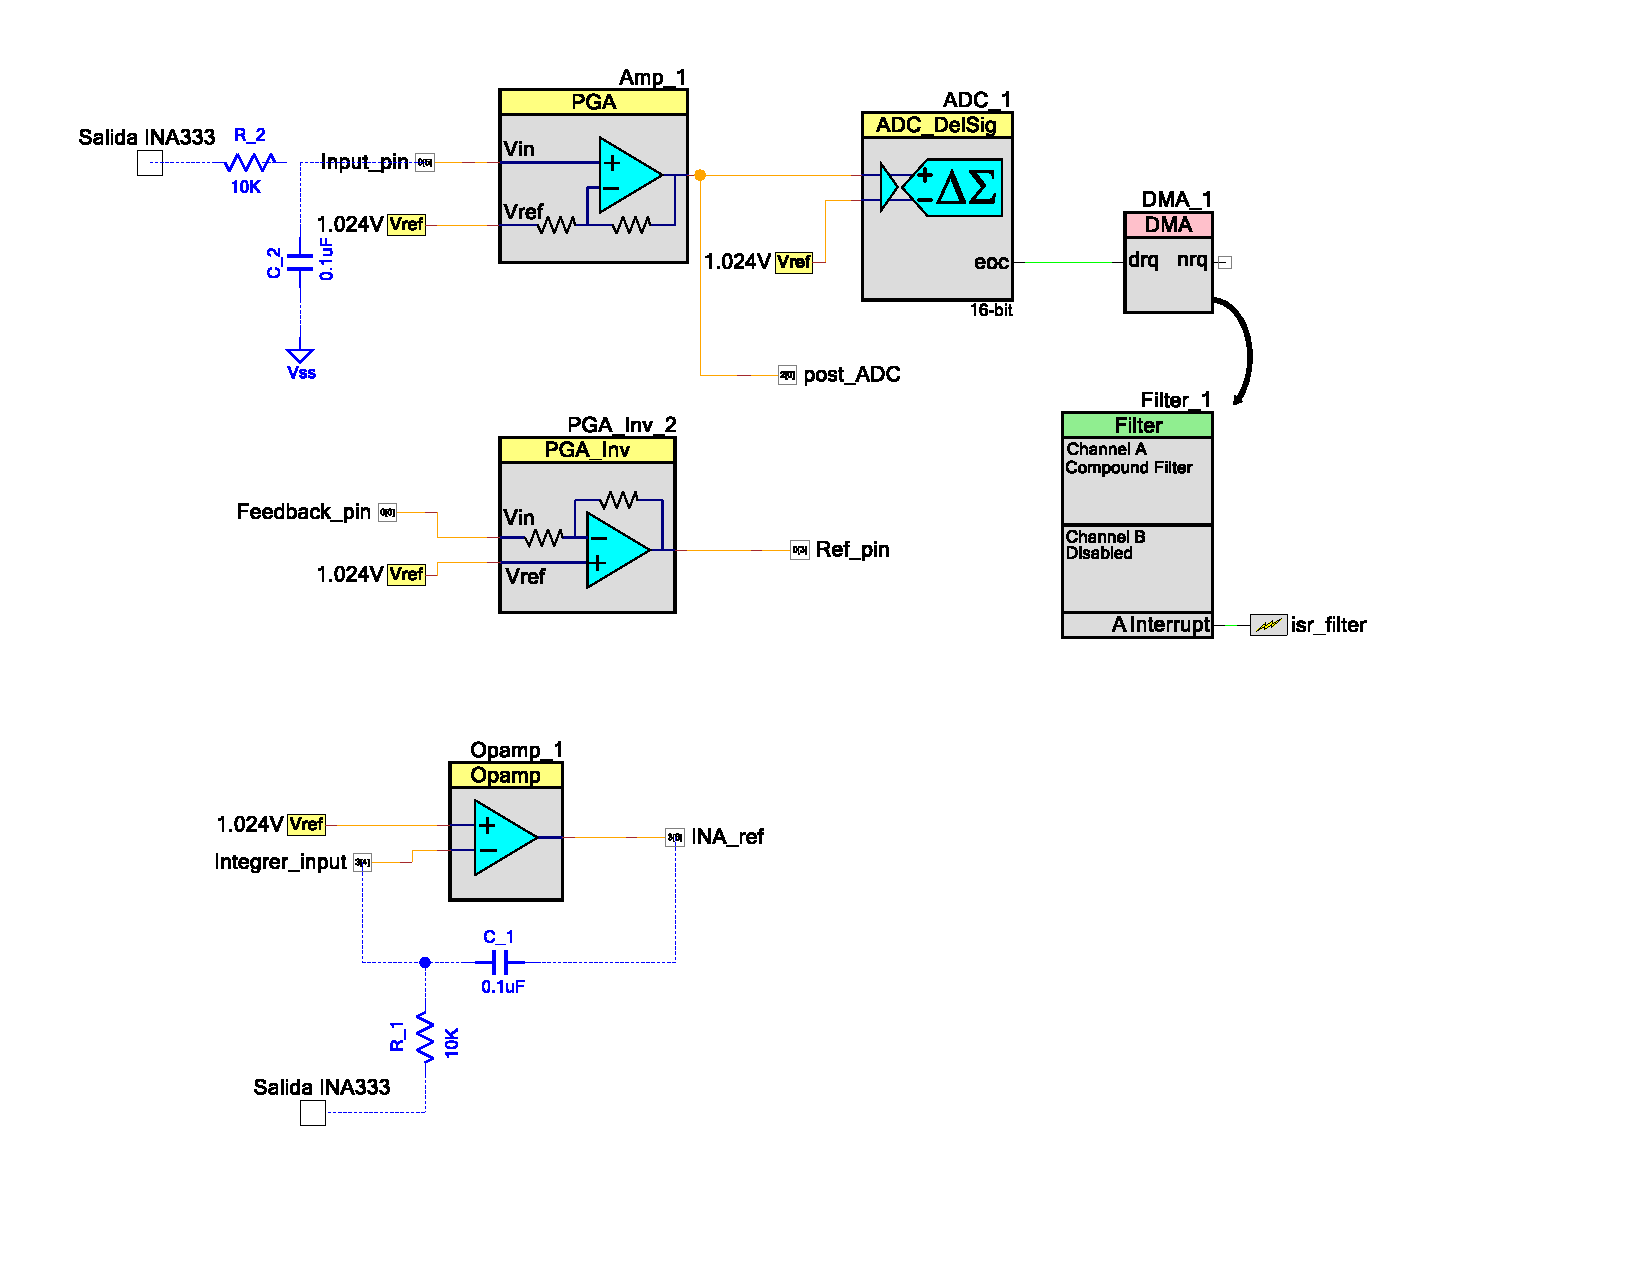
\includegraphics[height=0.85\textwidth , angle=90]{imagenes/hardware_psoc}
\caption{Configuración hardware del \acrshort{psoc} para la adquisición de la señal}
\end{figure}

\newpage

\begin{figure}[!ht]
\center
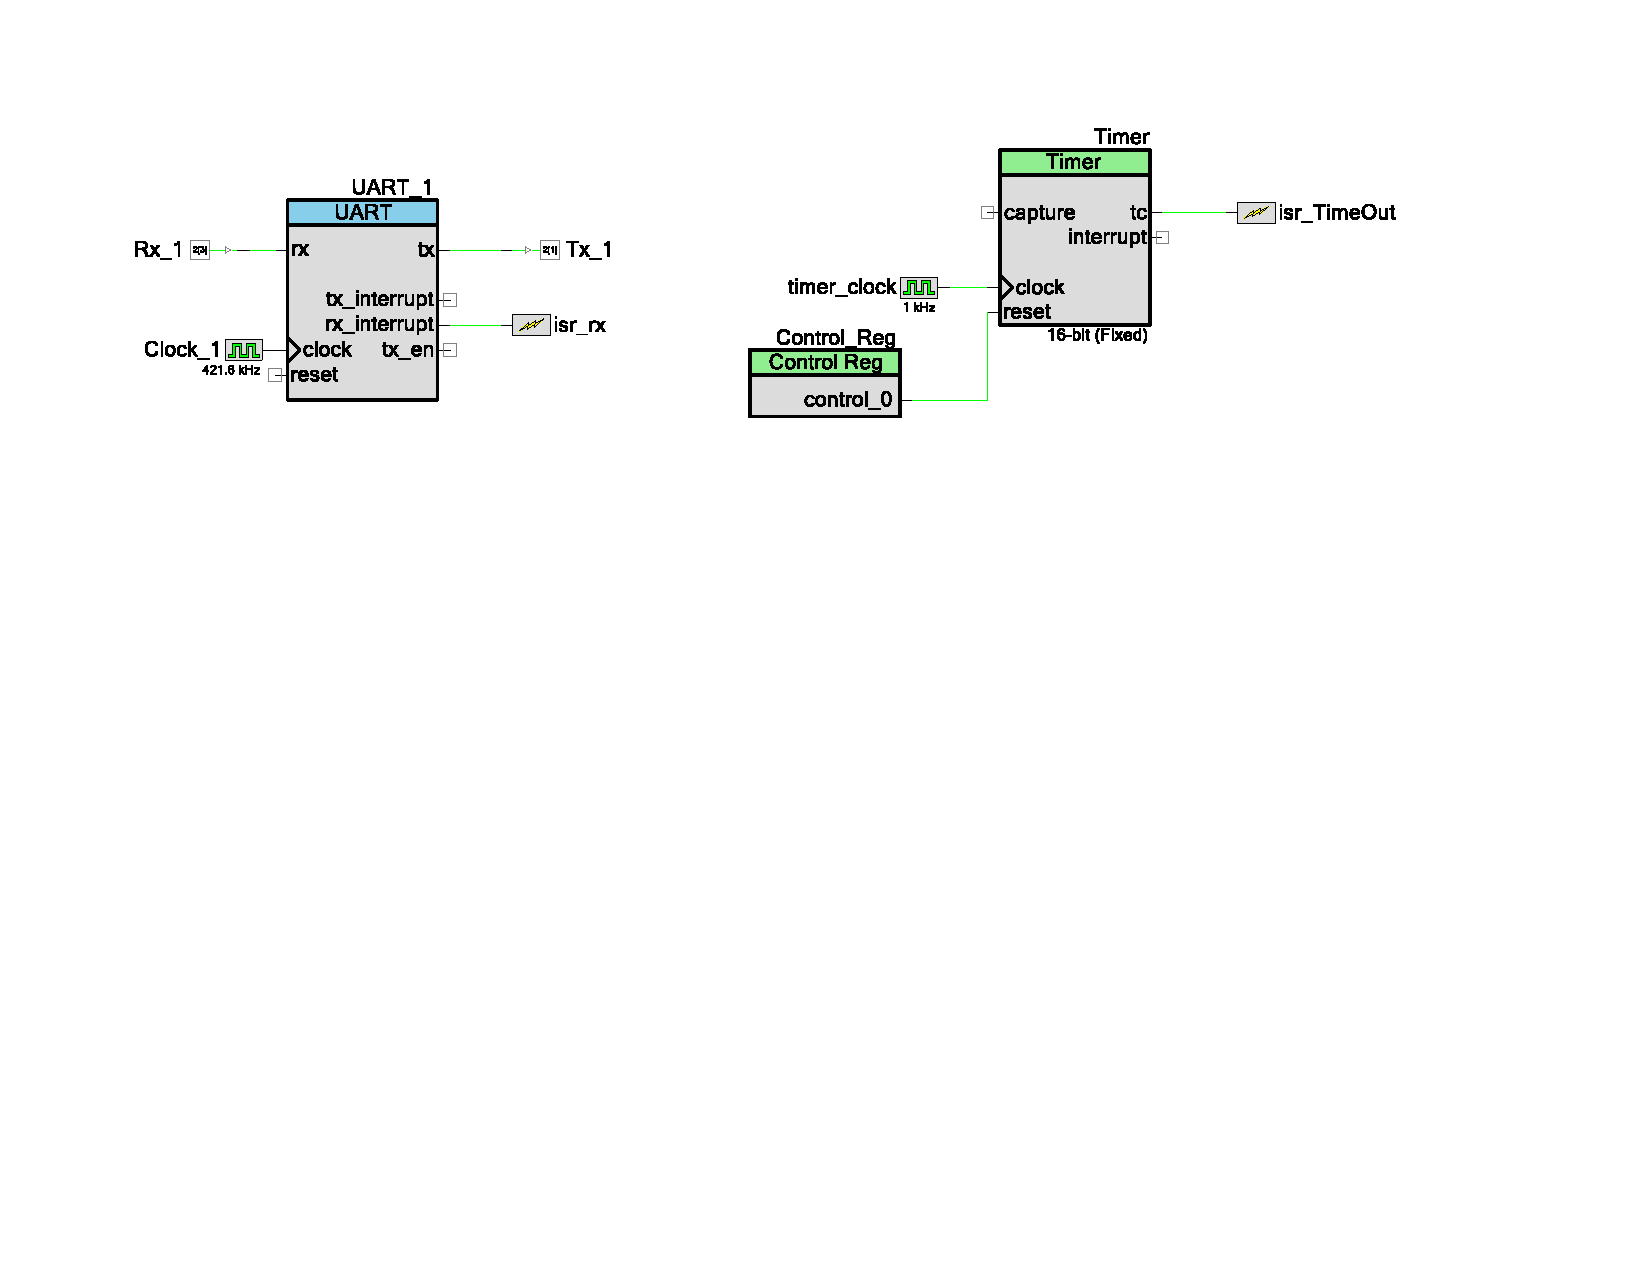
\includegraphics[width=0.92\textheight , angle=90]{imagenes/hardware_psoc_2}
\caption{Configuración hardware del \acrshort{psoc} para el modo de bajo consumo}
\end{figure}

\newpage
\section{Menús aplicación Android}

En este apéndice se muestran los menús de la aplicación desarrollada y la secuencia de mensajes al inicio para una mejor comprensión del funcionamiento de la misma. En las figuras se va mostrando la secuencia de mensajes y menús que van surgen en la interacción con la aplicación



\begin{figure}[!ht]
\center
\includegraphics[scale=0.3]{imagenes/App/Aviso_blue}
\caption{Configuración hardware del \acrshort{psoc} para el modo de bajo consumo}
\end{figure}

\begin{figure}[!ht]
\center
\includegraphics[scale=0.3]{imagenes/App/Permiso_blue}
\caption{Configuración hardware del \acrshort{psoc} para el modo de bajo consumo}
\end{figure}

\begin{figure}[!ht]
\center
\includegraphics[scale=0.3]{imagenes/App/Dispositivos}
\caption{Configuración hardware del \acrshort{psoc} para el modo de bajo consumo}
\end{figure}

\begin{figure}[!ht]
\center
\includegraphics[scale=0.3]{imagenes/App/Aviso_relleno_campos}
\caption{Configuración hardware del \acrshort{psoc} para el modo de bajo consumo}
\end{figure}


%%

